Kassow Robots teach pendant is a graphical user interface which allows users
to control robot arm and \hyperref[acro:HW]{HW} equipment, build and run programs and configure robot installation setup.
It is intended to be intuitive as it comes with familiar design of a tablet. The main screen interface is based
on a double pane layout between which there is a command box. The command box provides access to basic building blocks,
loaded CBun devices, and subroutines defined by the operator. These commands can be dragged and dropped into the program
tree. \cite[page 15]{kassow-software-manual}
There is a control mode in the bottom which can set the master speed or launch the program and control the execution process. (pause, continue, terminate). The program tree view is where the robot program is built in an intuitive graphical way.
A program tree contains at least one sequence. A sequence contains a number of commands that are executed sequentially.
For separate sequences, the commands are executed simultaneously and asynchronously. \cite[page 20]{kassow-software-manual}


\begin{figure}[h]
    \centering
    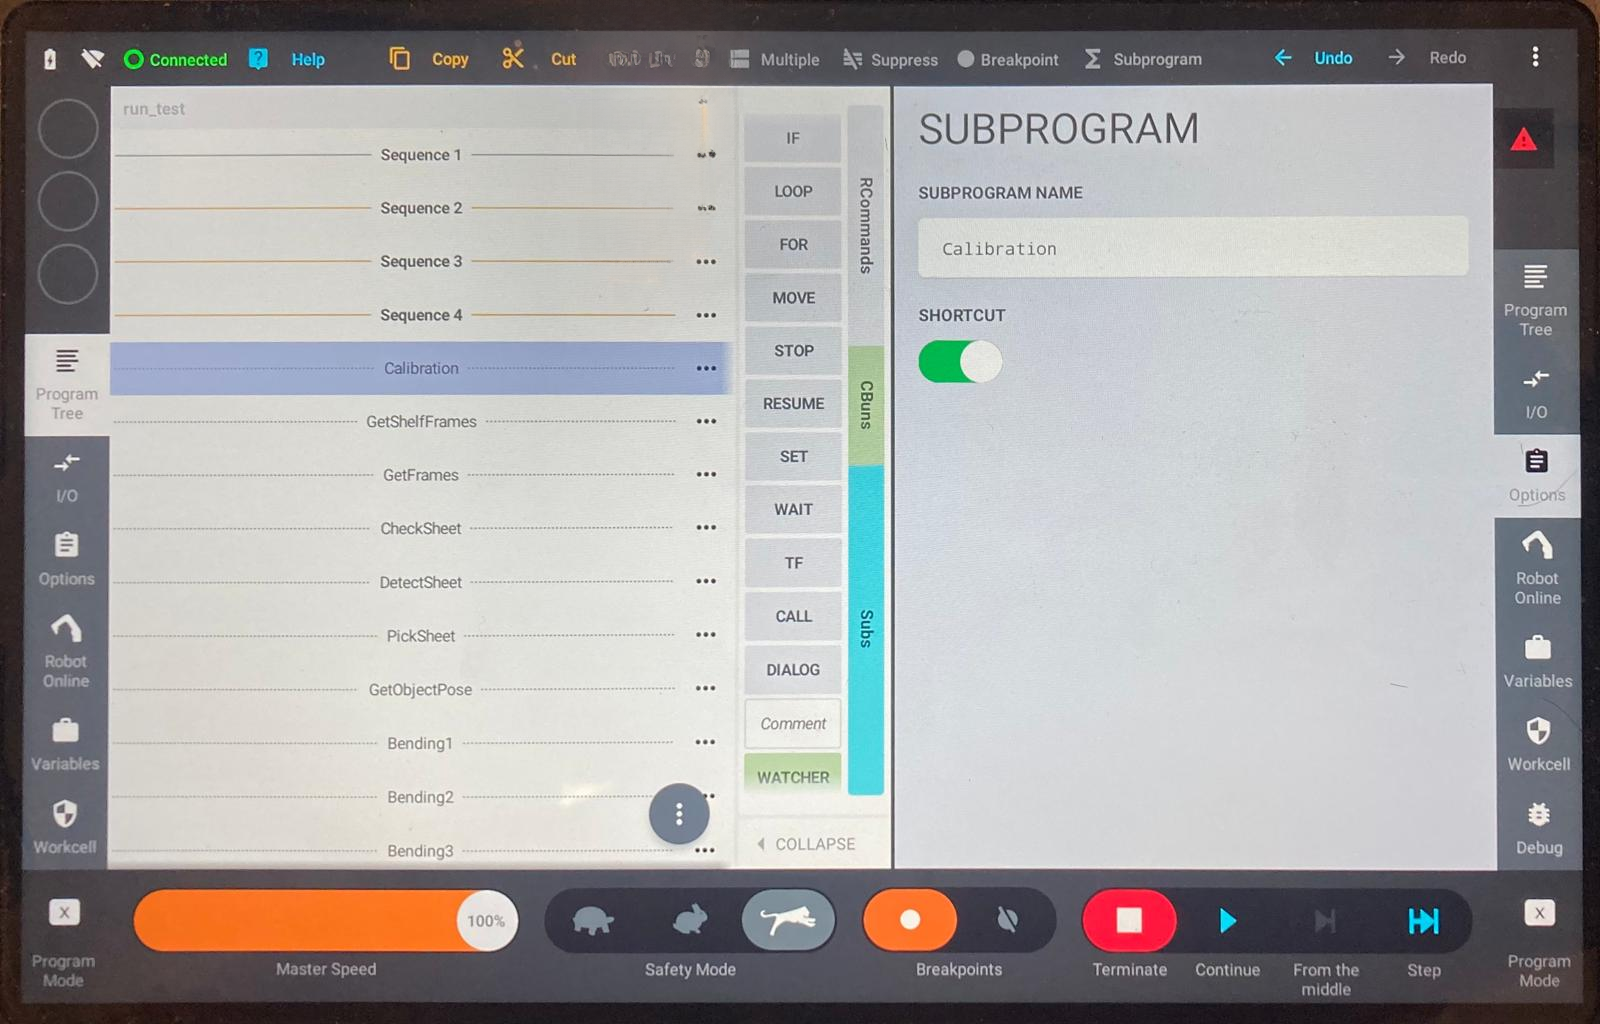
\includegraphics[width=\textwidth]{figures/programtree.png}
    \caption{Programming in teach pendant for a sheet metal part variant}
    \label{fig:programtree}
\end{figure}


The programming of \hyperref[acro:KR]{KR1410} is done in the program tree for one sheet metal part variant.
It is done to test the bending process using the \hyperref[acro:KR]{KR1410}.
The program tree of the workcell consists of four sequences which runs in parallel.
Sequence 1 is the main program which runs all the pick-place and bending operations.
Sequence 2 and 3 looks for a signal from \hyperref[acro:PLC]{PLC} for pausing and terminating the current program
respectively. Sequence 4 controls the robotic and unloading station grippers using a push button
for manual operation of the gripper in case of emergency.

The robot is programmed using a number of subprograms such that a subprogram
can be quickly imported in the sequence and is intuitive to understand as shown in figure \ref{fig:programtree}
Besides normal RCommands like IF, LOOP, FOR, MOVE, WAIT and so on, there are a number of CBun devices
from Kassow Robots
imported like the IK, FK and WATCHER devices. IK is used to get the inverse
kinematics from a pose and FK is used to get the forward kinematics
from a joint configuration.
Custom made CBuns modules for \hyperref[acro:VISOR]{VISOR}\textsuperscript{\textregistered}
are also used for auto-calibration and for getting the pose in the
robot frame of a detected object in the workspace using the \hyperref[acro:VISOR]{VISOR}\textsuperscript{\textregistered} vision sensor.

